% Editable standalone vector figure extracted from spectra.tex.
% Source slide 22; figure 21; native embedded fonts.
% Compile with LuaLaTeX from this directory, or run ../export_figures.py.
\documentclass[tikz,border=0pt]{standalone}
% Shared editable preamble for standalone, Nature-style vector figures.
% Text remains embedded and searchable. This is a house-style target, not a
% claim of acceptance or of satisfying every journal's submission checklist.
\usepackage{fontspec}
\setmainfont{LiberationSans}[
  Path=../../shared/assets/,Extension=.ttf,
  UprightFont=*-Regular,BoldFont=*-Bold,ItalicFont=*-Italic,BoldItalicFont=*-BoldItalic]
\setsansfont{LiberationSans}[
  Path=../../shared/assets/,Extension=.ttf,
  UprightFont=*-Regular,BoldFont=*-Bold,ItalicFont=*-Italic,BoldItalicFont=*-BoldItalic]
\setmonofont{LiberationSans}[
  Path=../../shared/assets/,Extension=.ttf,
  UprightFont=*-Regular,BoldFont=*-Bold,ItalicFont=*-Italic,BoldItalicFont=*-BoldItalic]
\usepackage{unicode-math}
\setmathfont{Latin Modern Math}
\DeclareMathSizes{5.9}{6}{5}{5}
\DeclareMathSizes{6}{6}{5}{5}
\usepackage{tikz}
\usetikzlibrary{arrows.meta,calc,positioning,patterns,decorations.pathreplacing,matrix}
\usepackage{graphicx}
\usepackage{xcolor}
\pagecolor{white}
\definecolor{ink}{HTML}{202020}
\definecolor{paper}{HTML}{FFFFFF}
\definecolor{muted}{HTML}{494949}
\definecolor{line}{HTML}{808080}
\definecolor{soft}{HTML}{F0F0F0}
\hyphenpenalty=10000\exhyphenpenalty=10000
\newcommand{\figurefont}{\sffamily\fontsize{5.9}{7.4}\selectfont}
\newcommand{\figuremathfont}{\sffamily\fontsize{6}{7.5}\selectfont}
\newcommand{\brandmedium}{\bfseries}
\renewcommand{\normalsize}{\figurefont}
\renewcommand{\small}{\figurefont}
\renewcommand{\footnotesize}{\figurefont}
\renewcommand{\scriptsize}{\figurefont}
\renewcommand{\tiny}{\figurefont}
\renewcommand{\large}{\figurefont}
\renewcommand{\Large}{\figurefont}
\renewcommand{\LARGE}{\figurefont}
\renewcommand{\huge}{\figurefont}
\renewcommand{\Huge}{\figurefont}
\tikzset{
  every path/.style={line width=.55pt},
  every node/.style={font=\figurefont,text=ink},
  arr/.style={-{Latex[length=1.5mm,width=1mm]},line width=.55pt,draw=ink},
  thinarr/.style={-{Latex[length=1.3mm,width=.9mm]},line width=.55pt,draw=ink},
  box/.style={draw=ink,line width=.55pt,fill=white,minimum height=.85cm,align=center,inner sep=3pt},
  ghost/.style={draw=muted,dashed,fill=soft},
  tag/.style={font=\figurefont,text=muted},
  equ/.style={font=\figuremathfont},
  small/.style={font=\figurefont},
  body/.style={font=\figurefont},
  tinytext/.style={font=\figurefont}
}
\newcommand{\txt}[4]{\node[anchor=north west,align=left,text width=#3cm] at (#1,#2) {#4};}
\newcommand{\smalltxt}[4]{\node[anchor=north west,align=left,text width=#3cm,small] at (#1,#2) {#4};}
\newcommand{\eqn}[4][6]{\node[anchor=north west,font=\figuremathfont] at (#2,#3) {$\displaystyle #4$};}
\newcommand{\diagramblock}[5]{\node[box,minimum width=#3cm,text width=#3cm,minimum height=#4cm] at (#1,#2) {#5};}
% Scale coordinates, not text: all labels retain one final publication size.
\newcommand{\spectrum}[3]{\begin{scope}[shift={(#1,#2)}]
  \draw[muted] (0,0)--({3.6*#3},0);
  \draw[muted] (0,0)--(0,{1.9*#3});
  \foreach \x/\h in {.25/.18,.49/.46,.68/1.42,.87/.37,1.08/.74,1.31/.31,1.57/1.78,1.76/.46,1.96/.19,2.17/1.1,2.37/.57,2.57/.31,2.88/.76,3.21/.23,3.4/.38}{
    \draw[ink] ({\x*#3},0)--({\x*#3},{\h*#3});}
  \foreach \x in {.6,1.2,1.8,2.4,3.0}{\draw[ink] ({\x*#3},0)--+(0,{-.06*#3});}
  \foreach \y in {.45,.9,1.35,1.8}{\draw[ink] (0,{\y*#3})--+({-.06*#3},0);}
  \foreach \x/\lab in {0/0,1.8/45,3.6/90}{\node[anchor=north,font=\figurefont] at ({\x*#3},{-.08*#3}) {\lab};}
  \foreach \y/\lab in {0/0,.9/0.5,1.8/1.0}{\node[anchor=east,font=\figurefont] at ({-.08*#3},{\y*#3}) {\lab};}
  \node[anchor=north east,font=\figurefont] at ({3.6*#3},{-.45*#3}) {$m/z$ (Th)};
  \node[anchor=south west,font=\figurefont] at (0,{1.96*#3}) {Relative intensity (a.u.)};
\end{scope}}
\newcommand{\molecule}[3]{\begin{scope}[shift={(#1,#2)}]
  \draw[ink] (0,{#3})--({.866*#3},{.5*#3})--({.866*#3},{-.5*#3})--(0,{-#3})--({-.866*#3},{-.5*#3})--({-.866*#3},{.5*#3})--cycle;
  \draw[ink] ({.68*#3},{.4*#3})--({.68*#3},{-.4*#3});
  \draw[ink] ({-.7*#3},{-.44*#3})--({-.02*#3},{-.83*#3});
  \draw[ink] ({-.7*#3},{.44*#3})--({-.02*#3},{.83*#3});
  \draw[ink] (0,{#3})--(0,{1.55*#3});
  \node[font=\figurefont] at (0,{1.77*#3}) {OH};
\end{scope}}
\newcommand{\peaktokens}[3]{\foreach \i in {0,...,5}{\pgfmathsetmacro{\xx}{#1+\i*.36}\draw[fill=#3,draw=ink] (\xx,#2) rectangle +(.24,.6);}}
\newcommand{\E}{\mathbb E}
\newcommand{\R}{\mathbb R}
\newcommand{\sg}{\operatorname{stopgrad}}
\newcommand{\LN}{\operatorname{LN}}
\newcommand{\softmax}{\operatorname{softmax}}

\begin{document}
\figurefont
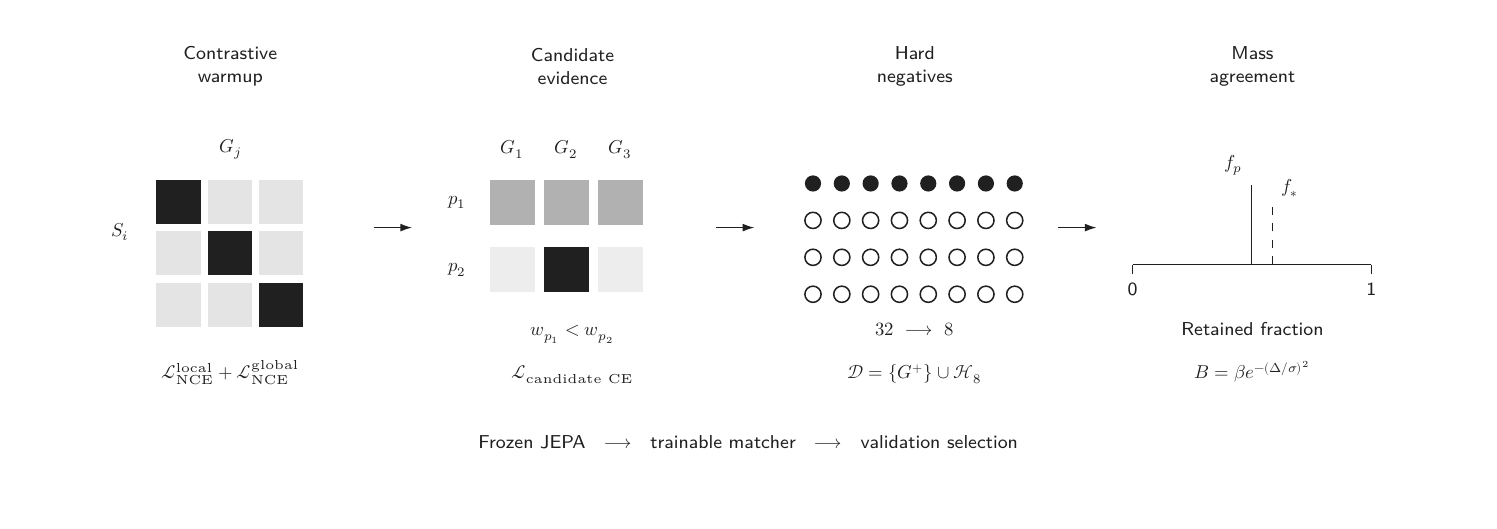
\begin{tikzpicture}[x=1cm,y=1cm,scale=1.14375,transform shape]
% Four stages; all mini-diagrams are schematic, not training measurements.
\foreach \x/\title in {2.25/Contrastive\\warmup,6.05/Candidate\\evidence,9.85/Hard\\negatives,13.60/Mass\\agreement}{
 \node[font=\figurefont,align=center,text width=3.15cm] at (\x,6.42) {\title};}
\foreach \x in {3.84,7.64,11.44}{\draw[arr] (\x,4.63)--+(.43,0);}

% Stage 1: positive pairs on the diagonal of an in-batch similarity matrix.
\node at (2.25,5.50) {$G_j$};
\node at (1.03,4.58) {$S_i$};
\foreach \r in {0,...,2}{\foreach \c in {0,...,2}{
 \pgfmathtruncatemacro{\shade}{ifthenelse(\r==\c,100,12)}
 \fill[ink!\shade] (1.43+\c*.57,5.16-\r*.57) rectangle +(.49,-.49);}}
\node[anchor=base,inner sep=0,font=\figurefont] at (2.25,2.95)
 {$\mathcal L_{\rm NCE}^{\rm local}+\mathcal L_{\rm NCE}^{\rm global}$};

% Stage 2: a common peak versus a peak that distinguishes the candidates.
\foreach \x/\label in {5.38/1,5.98/2,6.58/3}{\node at (\x,5.50) {$G_{\label}$};}
\node at (4.77,4.91) {$p_1$};\node at (4.77,4.16) {$p_2$};
\foreach \x in {5.13,5.73,6.33}{\fill[ink!35] (\x,4.66) rectangle +(.5,.5);}
\foreach \x in {5.13,6.33}{\fill[ink!8] (\x,3.91) rectangle +(.5,.5);}
\fill[ink] (5.73,3.91) rectangle +(.5,.5);
\node[anchor=base,inner sep=0] at (6.05,3.43) {$w_{p_1}<w_{p_2}$};
\node[anchor=base,inner sep=0,font=\figurefont] at (6.05,2.95) {$\mathcal L_{\rm candidate\ CE}$};

% Stage 3: score up to 32 sampled negatives; retain the hardest eight.
\foreach \r in {0,...,3}{\foreach \c in {0,...,7}{
 \ifnum\r=0
  \fill[ink] (8.72+\c*.32,5.12-\r*.41) circle (.09);
 \else
  \draw[draw=ink,line width=.55pt,fill=white] (8.72+\c*.32,5.12-\r*.41) circle (.09);
 \fi}}
\node[anchor=base,inner sep=0] at (9.85,3.43) {$32\ \longrightarrow\ 8$};
\node[anchor=base,inner sep=0,font=\figurefont] at (9.85,2.95) {$\mathcal D=\{G^+\}\cup\mathcal H_8$};

% Stage 4: agreement between peak and candidate retained-mass fractions.
\draw[ink,line width=.55pt] (12.27,4.22)--(14.92,4.22);
\foreach \x/\lab in {12.27/0,14.92/1}{
 \draw[ink,line width=.55pt] (\x,4.22)--+(0,-.10);
 \node[anchor=north] at (\x,4.09) {\lab};}
\draw[ink,line width=.55pt] (13.59,4.22)--(13.59,5.10);
\draw[ink,line width=.55pt,dashed] (13.82,4.22)--(13.82,4.86);
\node[anchor=south east] at (13.57,5.13) {$f_p$};
\node[anchor=south west] at (13.84,4.89) {$f_*$};
\node[anchor=base,inner sep=0] at (13.60,3.43) {Retained fraction};
\node[anchor=base,inner sep=0,font=\figurefont] at (13.60,2.95) {$B=\beta e^{-(\Delta/\sigma)^2}$};

\node[font=\figurefont] at (8.0,2.25)
 {Frozen JEPA\quad$\longrightarrow$\quad trainable matcher\quad$\longrightarrow$\quad validation selection};
% Fixed canvas: 183 x 60.046875 mm. No clipping: overflow is audited.
\pgfresetboundingbox
\path[use as bounding box] (0,1.6) rectangle (16,6.85);
\end{tikzpicture}
\end{document}
